\documentclass[11pt,a4paper]{article}
\usepackage[margin=2.2cm]{geometry}
\usepackage[T1]{fontenc}
\usepackage{lmodern,microtype}\emergencystretch=2em
\usepackage{amsmath,amssymb}
\usepackage{graphicx,booktabs,multirow,xcolor,float,caption,subcaption}
\usepackage[most]{tcolorbox}
\usepackage{enumitem}
\usepackage[colorlinks=true,linkcolor=blue!50!black,urlcolor=blue!50!black]{hyperref}
\definecolor{ink}{HTML}{1F4E79}
\newtcolorbox{verdict}[1][]{colback=ink!5,colframe=ink,fonttitle=\bfseries,title=#1}
\newcommand{\ok}{\textcolor{green!50!black}{\textbf{reproduced}}}
\newcommand{\partly}{\textcolor{orange!80!black}{\textbf{partly reproduced}}}
\newcommand{\notrep}{\textcolor{red!70!black}{\textbf{not reproduced}}}
\newcommand{\BuildSecondsBig}{8}
\newcommand{\DemoDfour}{140 (range 132--148)}
\newcommand{\DemoDfive}{115 (range 112--117)}
\newcommand{\RFRecallHalf}{30\%}
\newcommand{\RFRecallTwo}{92\%}
\newcommand{\OursTthree}{47.1}
\newcommand{\NTthree}{20}
\newcommand{\QualityFindings}{(i) \emph{Table III reproduces}: the faithful loop reaches 47.1 gates on average (paper: 45 on its single circuit), against
127 for Qiskit L3. (ii) \emph{Table IV}: we obtain 36.8 gates (paper: 72), so the method is even stronger than reported here.
(iii) Qiskit 2.5 is much stronger than the version used in the paper (L3: 127 vs.\ 176 and 104 vs.\ 153). (iv) \emph{Table V does not
reproduce}: at 15 qubits the method (335.9 gates, 213 CZ) only ties Qiskit L3 (332.1 gates, 213.5 CZ), whereas the paper reports
293 vs.\ 313. Most random 15-qubit gate pairs act on disjoint wires, so there is little for 3-wire windows to do that Qiskit's
commutation analysis does not already do. These runs also reached the 400\,s cap, so a longer budget could help somewhat.
(v) Two-qubit gates are reduced proportionally (3q ion: 43 $\to$ 18.9 RXX; Qiskit L3: 29.9). All outputs were verified equivalent to their inputs.
}
\newcommand{\NJPFindings}{\textbf{Findings.} Our faithful port gives 78.8 (ion trap) and 76.0 (IBM-style) gates on average, \emph{better} than the published
111 and 107. Qiskit 2.5 L3 gives 164.9 and 140.9. The difference to the published numbers is plausibly due to the database used
(ours: 24-op depth 5 / 15-op depth 6, unstated in the paper) and run time. The qualitative claim, that the method clearly beats Qiskit on
few-qubit random circuits, reproduces. The extension paper shows that an exact convex-window optimiser reaches 56.7 / 59.1 on the
same benchmark in $\sim$6\,s per circuit.
}
\newcommand{\HardwareFindings}{\textbf{Findings.} At transpiler levels 0 and 1 the reduced circuits are closer to the ideal distribution on both chips
(Brisbane L0: TVD 0.059 $\to$ 0.041, better on 22/30 circuits; Kyiv L0: 0.024 $\to$ 0.018, 20/30), and the newer Kyiv calibration
is less noisy than Brisbane. Both observations match the paper's Fig.~9. At level 3, however, Qiskit consolidates every 2-qubit
block and re-synthesises it, so long and short circuits compile to the same $\approx1.1$ two-qubit gates and the advantage
vanishes (Brisbane 0.018 vs.\ 0.019; Kyiv 0.012 vs.\ 0.012). Plain Qiskit level 3 on the \emph{long} circuit beats the reduced circuit at
level 1 (0.018 vs.\ 0.037 on Brisbane). The paper's hardware evidence therefore depends on an unreported transpiler setting.
Its native-op counts (156 vs.\ 34 on Brisbane) are consistent with level 0/1 compilation by an older Qiskit. Our reduced
circuits average 5.4 gates (paper: 8).
}

\makeatletter\newcommand{\tabinput}[1]{\@@input #1 }\makeatother

\title{\textbf{Reproduction report}\\[4pt]\large ``Optimization Driven Quantum Circuit Reduction''\\(Rosenhahn, Osborne, Hirche, arXiv:2502.14715)}
\author{Reproduction based on the authors' MATLAB demo code, ported to Python}
\date{}
\begin{document}
\maketitle\sloppy

\begin{verdict}[Summary]
\begin{tabular}{p{4.3cm}p{2.4cm}p{7.4cm}}
\textbf{Claim}&\textbf{Status}&\textbf{Comment}\\\midrule
Table I (compute-graph sizes)&\ok&All 22 node/edge counts identical.\\
Fig.~1 (Bell example)&\ok&Both circuits equal $\mathrm{CNOT}(H\otimes I)$; 4 gates is optimal.\\
Fig.~4 (40-gate 2q example)&\ok&$40\to4$. But the paper's own 4-gate output has optimum 2.\\
Fig.~6/7, Table II (V1 $>$ V2 $>$ V3 time)&\partly&Ordering V1 $\gg$ V2 holds. V3 beats V2 \emph{only} with a tuned
forest threshold; at the default 0.5 it is slower than V2.\\
Table III (ion trap 3q)&\ok&With the 24-op depth-5 database: \OursTthree\ gates vs.\ paper 45.\\
Table IV/V (IBM-style 3q/15q)&\partly&3q: reproduced and stronger (36.8 vs.\ paper 72). 15q: the method only ties Qiskit 2.5 L3 (335.9 vs.\ 332.1).\\
NJP 4q statistics&\ok&Faithful port: 78.8 / 76.0 gates (published 111 / 107); Qiskit L3: 164.9 / 140.9.\\
Fig.~9 (IBM hardware)&\partly&Noisy-simulator reproduction: the effect exists at transpiler levels 0/1 and essentially
vanishes at level 3.\\
\end{tabular}
\end{verdict}

\section{What ``the code given'' is, and how we ran it}
The authors ship a MATLAB demo, linked only in the journal version's ref.~[38]
(\url{https://www.tnt.uni-hannover.de/en/staff/rosenhahn/QCOptimDemo.zip}; the arXiv version has no link). It is \texttt{QCOptimDemo}, with \texttt{FullQCGraphIOn3\_4.m},
\texttt{optimCodeGMode1DComp.m} and helpers). It implements the compute-graph database and the V2 optimiser only;
V1 and V3 are described in the paper but not included. The demo requires MATLAB's Quantum Computing Support Package,
which is not available to us (and is not Octave compatible). We therefore ported it line by line to Python
(\texttt{qcr}):
\begin{itemize}[nosep]
\item \texttt{gates.py}: MATLAB gate conventions ($R_P(\theta)=e^{-i\theta P/2}$, qubit 1 most significant, $U=O(L)\cdots O(1)$), pools
  in the order of \texttt{QoperatorsIon1.m}.
\item \texttt{unitary.py}: \texttt{compare.m} verbatim (least-squares phase, spectral norm), plus a canonical
  phase-normalised hash key.
\item \texttt{compute\_graph.py}: the full compute graph (BFS), parent pointers = shortest-path factorisations.
\item \texttt{reducer.py}: the optimiser loop of \texttt{optimCodeGMode1DComp.m}: shuffle w.p.\ 0.7 (each commuting pair
  w.p.\ 0.6), block start/length sampling identical to MATLAB's \texttt{randi} calls, $\le3$-wire rejection, wire
  reduction/lift, \texttt{simplereduce} including its loop bounds, tolerance $10^{-3}$, database without the identity.
  V2 lookups exist in two modes: \texttt{scan} (the MATLAB linear scan over entries shorter than the block) and \texttt{hash}
  (an $O(1)$ dictionary; same replacements, used where only output quality matters).
\item V1 (random sampling, 300 candidate words per block) and V3 (random forest, 50 trees, features = remapped token
  sequence + token histogram + length; labels from the exact database, as the paper describes) were implemented from the paper's text.
\end{itemize}
Every reduced circuit in every experiment was checked for equivalence with its input (dense unitary for $n\le5$,
random-state test for $n=15$). \textbf{All checks passed}; the maximal unitary deviation was $\sim10^{-12}$.
The authors' own demo output (\texttt{longcode10}$\to$\texttt{shortcode10}, $300\to140$ gates, 5 qubits) is also exactly
equivalent once the 4-decimal angles in the QASM file are snapped to $\pm\pi/2$.

Hardware: 8-core laptop, Python 3.14, NumPy 2.3, Qiskit 2.5, qiskit-aer 0.17, qiskit-ibm-runtime fake backends.
Timing experiments ran 8 processes in parallel; all four variants of a given circuit ran concurrently, so
relative comparisons are fair, but absolute times are not comparable with the authors' MATLAB numbers.

\section{Table I: compute graphs}
Node counts for 2 qubits / 14 operators (depth 1--6) and 3 qubits / 24 operators (depth 1--5) are \emph{identical} to the
paper, and so are the edge counts (which follow $E(d)=N(d{-}1)\cdot|\mathcal{OP}|$). The operator counts 14/24 imply the pool
contains $\mathrm{RXX}(\pm\pi/2)$. The demo code uses only $+\pi/2$ (13/21 operators), which gives smaller graphs
(3 qubits, depth 4: 12,441 nodes). Building the largest graph (137,572 nodes) takes \BuildSecondsBig\,s in Python.
An independent exact engine (Clifford tableaux, see the extension paper) gives the same counts.

\section{Figures 1, 4, 5: worked examples}
\begin{itemize}[nosep]
\item Fig.~1: both the 8-gate naive and the 4-gate optimised Bell circuits equal $\mathrm{CNOT}\,(H\otimes I)$ to $10^{-13}$.
  Exhaustive search shows no 3-gate circuit exists.
\item Fig.~4 analogue (2 qubits, 40 random gates, 2-qubit depth-6 database): $40\to34\to26\to24\to20\to18\to16\to8\to4$.
  The paper's figure also ends at 4. However, the paper's displayed final circuit
  $\mathrm{RXX}(\frac\pi2)\mathrm{RXX}(\frac\pi2)\mathrm{RZ}_2(\frac\pi2)\mathrm{RZ}_2(-\frac\pi2)$ contains an inverse pair that
  \texttt{simplereduce} cannot see (it never checks the last pair), and the database cannot remove it (identity excluded).
  Its optimum is 2. Note also that every step in our trace removes an even number of gates. For two qubits this is
  forced (gate-count parity is invariant, see the extension paper). The paper's Fig.~4 shows a $6\to3$ replacement, so it
  must have used a pool different from the one stated.
\item Fig.~5 analogue (3 qubits, 200 gates): $200\to36$ in 31 replacements.
\item Authors' demo circuit (\texttt{longcode10}, 5 qubits, 300 gates): authors' output 140 gates. Our port with the demo's
  21-op depth-4 database gives \DemoDfour; with the 24-op depth-5 database \DemoDfive\ (5 seeds each).
\end{itemize}

\section{Table II, Figs.~6--7: V1 vs.\ V2 vs.\ V3}
\textbf{Protocol} (unspecified in the paper; we follow the demo): 100 random 5-qubit ion-trap circuits of length 100,
3-qubit depth-4 database (12,441 entries; linear-scan lookup $\approx$10\,ms), target length 60, cap 600\,s.
V3 is run with the standard majority-vote threshold (0.5) and with a recall-oriented threshold (0.2).
\begin{table}[H]\centering\small
\begin{tabular}{lrrrrrrr}\toprule
Variant&runs&mean (s)&std (s)&median (s)&reached&attempts&lookups\\\midrule
\tabinput{../../results/tex/table2.tex}
\bottomrule\end{tabular}
\caption{Our Table II. Paper: V1 199$\pm$352\,s, V2 55$\pm$96\,s, V3 38$\pm$40\,s. ``reached'' = runs that hit the target
within 600\,s.}
\end{table}
\begin{figure}[H]\centering
\begin{subfigure}{0.49\textwidth}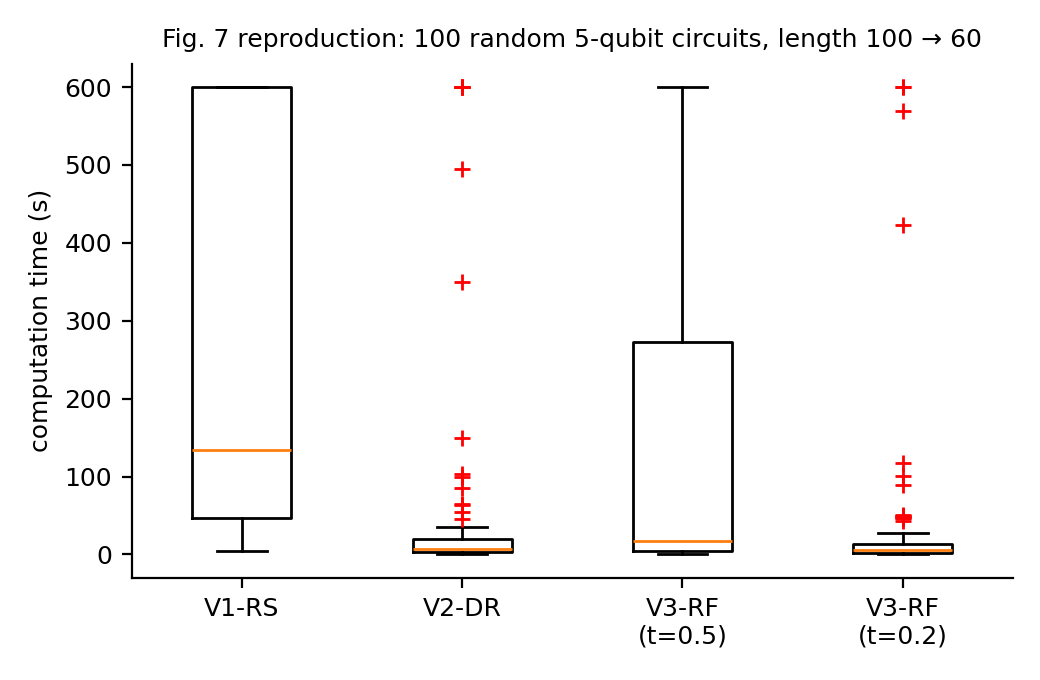
\includegraphics[width=\textwidth]{../../figures/repro_boxplot.png}\end{subfigure}
\begin{subfigure}{0.49\textwidth}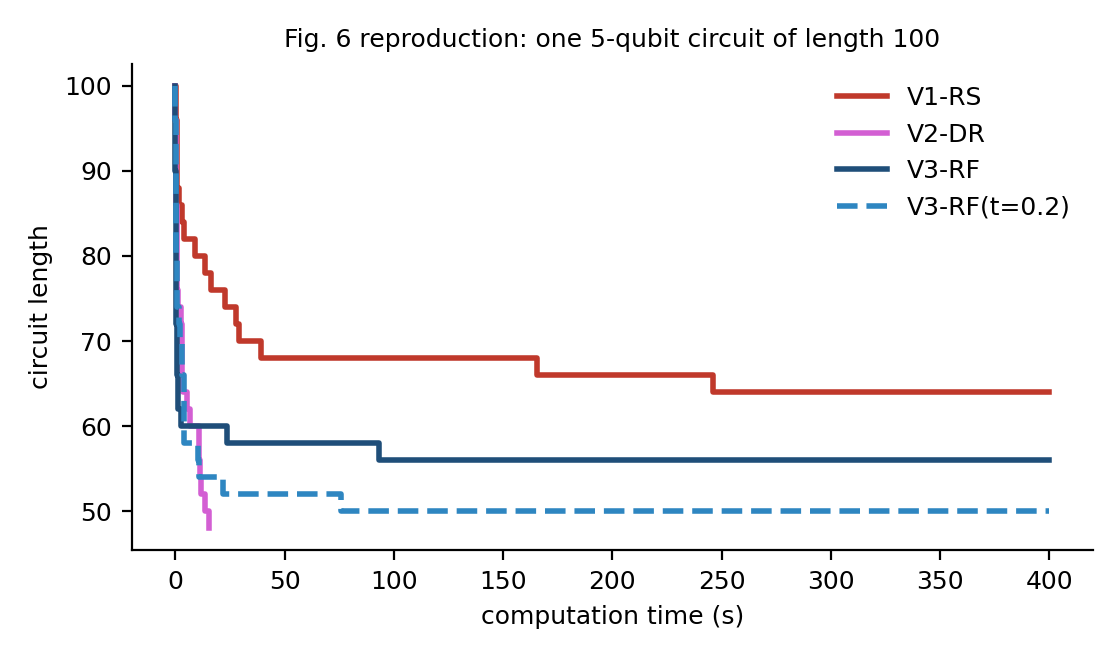
\includegraphics[width=\textwidth]{../../figures/repro_convergence.png}\end{subfigure}
\caption{Left: Fig.~7 reproduction. Right: Fig.~6 reproduction (single circuit, target 48, cap 400\,s). On this circuit V2 reaches
the target in 15\,s, while V1 (64), V3 at threshold 0.5 (56) and V3 at 0.2 (50) stall. Single-circuit curves are anecdotal; the 100-circuit
statistics on the left are the meaningful comparison.}
\end{figure}
\textbf{Findings.} (i) V1 is clearly slowest and has the heaviest tail, as in the paper. (ii) The database (V2) gives a large
speed-up. (iii) The forest's recall decides V3. On held-out blocks it predicts ``reducible'' for only
\RFRecallHalf\ of truly reducible blocks at threshold 0.5 (\RFRecallTwo\ at 0.2). At 0.5 it throws away most reductions
and needs $\sim$40$\times$ more attempts, and so is \emph{slower} than V2. At 0.2 it is the fastest variant, as the paper reports.
The paper does not report the threshold or the classifier's accuracy, so its V3 result can be reproduced only after
tuning. (iv) Replacing the linear scan by a hash lookup (0.03\,ms instead of 10\,ms) makes V2 faster than any V3
configuration, removing the reason for V3.

\section{Tables III--V: comparison with Qiskit}
Circuits are uniformly random native-gate strings (this matches the paper's gate proportions). ``Ours'' = faithful
V2 loop with hash lookup, stopped after 100,000 consecutive failed attempts (or 400\,s). Database: ion trap, 24-op depth 5
(Table I); IBM-style ($\mathrm{RX},\mathrm{RZ}(\pm\frac\pi2)$, CZ), 15-op depth 6 (109,639 entries). With the 21-op depth-4 demo
database, the 3-qubit ion-trap result stalls at $\approx76$ gates instead of $\approx42$. The paper does not state
which database was used, but only the larger one reproduces its numbers.
Columns: first circuit (as in the paper), then mean$\pm$std over all circuits.
\begin{table}[H]\centering\scriptsize
\begin{tabular}{l rrrr r | rrrr r}\toprule
&\multicolumn{5}{c|}{circuit 1}&\multicolumn{5}{c}{mean $\pm$ std over \NTthree\ circuits}\\
Method&rx&ry&rz&rxx&total&rx&ry&rz&rxx&total\\\midrule
\tabinput{../../results/tex/quality_T3_ion_3q.tex}
\bottomrule\end{tabular}
\caption{Table III reproduction (ion trap, 3 qubits, 300 gates). Paper: original 300, Qiskit L3 176, ours 45.}
\end{table}
\begin{table}[H]\centering\scriptsize
\begin{tabular}{l rrr r | rrr r}\toprule
&\multicolumn{4}{c|}{circuit 1}&\multicolumn{4}{c}{mean $\pm$ std}\\
Method&rx&rz&cz&total&rx&rz&cz&total\\\midrule
\multicolumn{9}{l}{\emph{Table IV: 3 qubits, 300 gates (paper: Qiskit L3 153, ours 72)}}\\
\tabinput{../../results/tex/quality_T4_nisq_3q.tex}
\midrule
\multicolumn{9}{l}{\emph{Table V: 15 qubits, 500 gates (paper: Qiskit L3 313, ours 293)}}\\
\tabinput{../../results/tex/quality_T5_nisq_15q.tex}
\bottomrule\end{tabular}
\caption{Tables IV and V reproduction (IBM-style gate set).}
\end{table}
\textbf{Findings.} \QualityFindings

\paragraph{NJP protocol (4 qubits, length 300; 30 random circuits per gate set, the first 30 of the 100 used in the extension paper).}
\begin{table}[H]\centering\scriptsize
\begin{tabular}{l rrrr r | rrrr r}\toprule
&\multicolumn{5}{c|}{circuit 1}&\multicolumn{5}{c}{mean $\pm$ std over 30 circuits}\\
Method&rx&ry&rz&rxx&total&rx&ry&rz&rxx&total\\\midrule
\tabinput{../../results/tex/quality_NJP_ion_4q.tex}
\bottomrule\end{tabular}

\smallskip
\begin{tabular}{l rrr r | rrr r}\toprule
Method&rx&rz&cz&total&rx&rz&cz&total\\\midrule
\tabinput{../../results/tex/quality_NJP_nisq_4q.tex}
\bottomrule\end{tabular}
\caption{Published (NJP Tables 6/7) ``ours'': ion trap 10/29/29/43 (total 111); IBM-style 45/19/43 (total 107).}
\end{table}
\NJPFindings

\section{Fig.~9: hardware experiment (noisy simulation of the same chips)}
We cannot access IBM Brisbane/Kyiv (both retired), so we use Qiskit's calibrated noise models \texttt{FakeBrisbane} and
\texttt{FakeKyiv}. Unlike the paper we use 30 random 2-qubit circuits of length 40 (each reduced with the 2-qubit
database), 4000 shots, and three transpiler levels. Metric: total-variation distance (TVD) of the measured distribution
from the ideal one.
\begin{table}[H]\centering\small
\resizebox{\textwidth}{!}{\begin{tabular}{llcccccc}\toprule
Chip&level&gates long/short&transpiled ops&2q gates (ECR)&TVD long&TVD short&short better\\\midrule
\tabinput{../../results/tex/hardware.tex}
\bottomrule\end{tabular}}
\caption{Fig.~9 reproduction, mean over 30 circuits ($\pm$ standard error).}
\end{table}
\begin{figure}[H]\centering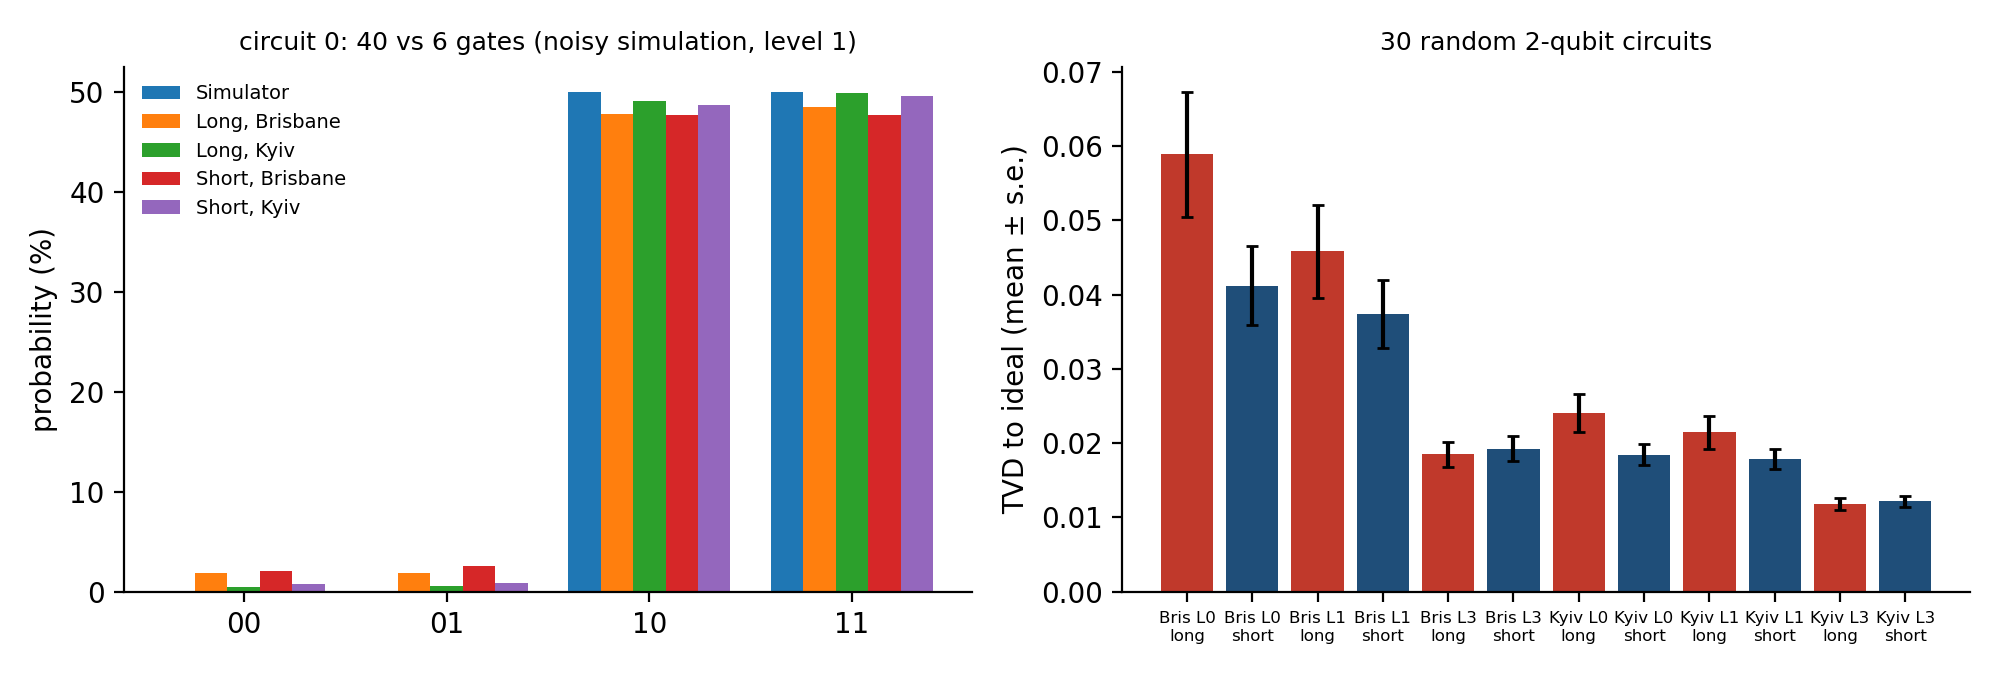
\includegraphics[width=\textwidth]{../../figures/repro_hardware.png}
\caption{Left: Fig.~9-style bars for one circuit. Right: TVD statistics.}\end{figure}
\HardwareFindings

\section{Bugs and undocumented choices found while reproducing}
\begin{enumerate}[nosep]
\item \texttt{simplereduce.m} never tests the last adjacent pair, and skips the pair following a deletion (visible in the paper's Fig.~4).
\item The database omits the identity (\texttt{Dists>0}), so identity blocks cannot be deleted by lookups.
\item Tolerances differ: paper $10^{-5}$, optimiser $10^{-3}$, graph builder $10^{-4}$.
\item Operator pools differ between Table I (14/24 ops) and the demo (13/21 ops), and the database used for Tables III--V is unstated.
  Only the larger one reproduces Table III.
\item Unspecified in the paper: qubit count and target length for Table II; forest features, size, threshold and accuracy;
  V1 sampling budget; transpiler level and shot count for the hardware experiment; which Qiskit version was used.
\item The hardware section's text names ``RX, RY and CX'', but the tables report RX, RZ, CZ.
\item The graph builder recomputes BFS distances only with probability 0.3 per step. This does not change the final counts.
\end{enumerate}

\section{How to rerun}
\begin{verbatim}
cd experiments
python3 exp_figures.py table1 examples demo convergence
python3 exp_table2_stats.py          # Table II / Fig. 7 (~2-3 h on 8 cores)
python3 exp_quality.py               # Tables III-V + NJP protocol
python3 exp_hardware.py              # Fig. 9 with FakeBrisbane / FakeKyiv
python3 make_assets.py               # tables/figures used in this report
\end{verbatim}
\end{document}
